\documentclass[border=10pt]{standalone}
\usepackage{tikz}
\usetikzlibrary{3d, arrows.meta, shadings, calc}

\begin{document}

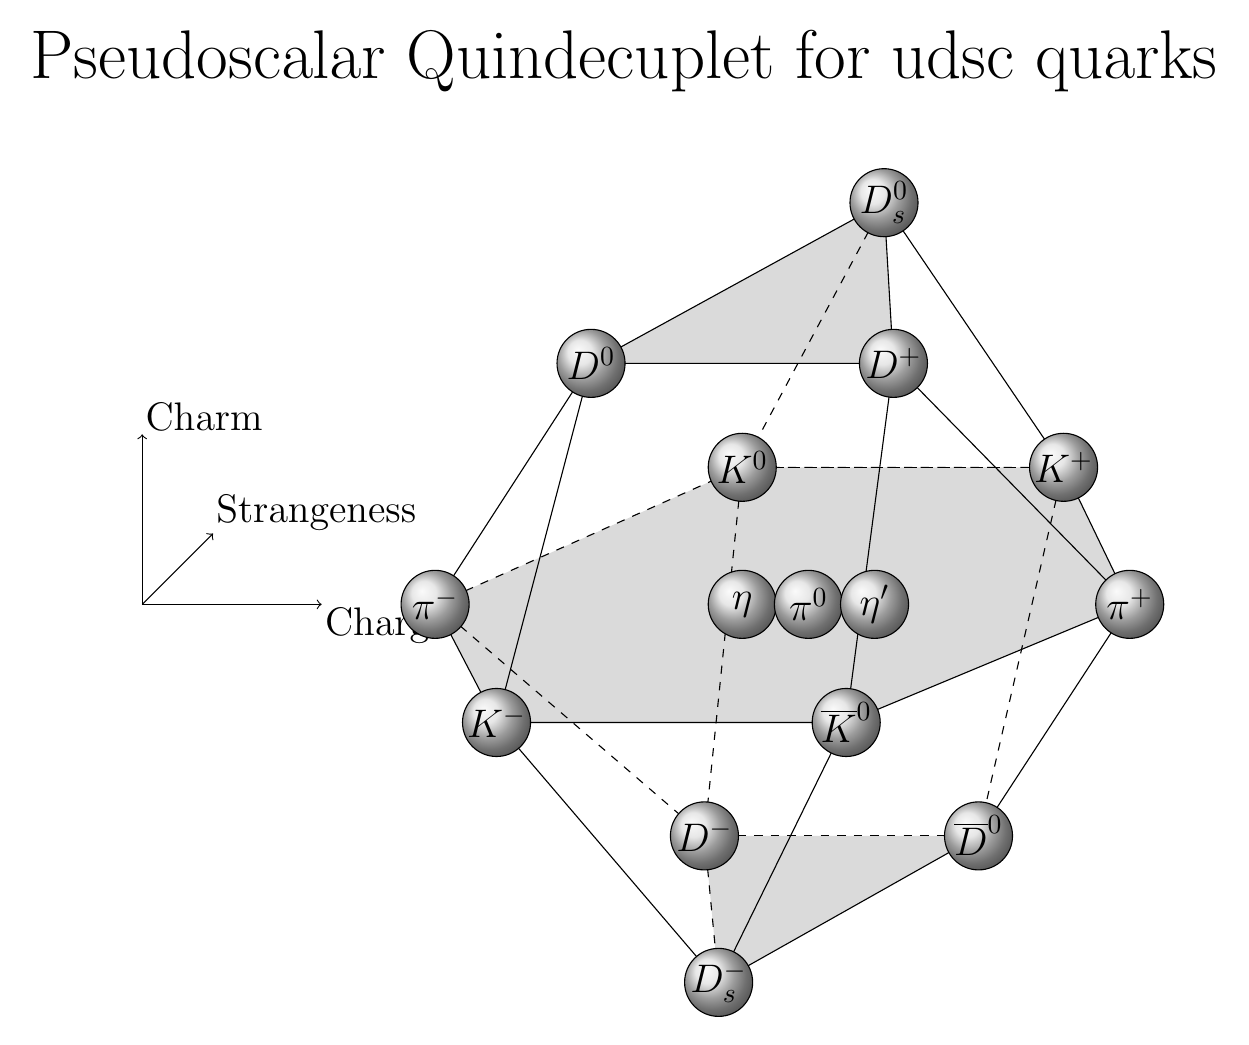
\begin{tikzpicture}[
    scale=1.2,
    every node/.style={font=\small, inner sep=1pt},
    axis/.style={->, >=to, thin},
    sphere/.style={ball color=gray!25, draw=black, thin},
    edge/.style={thin},
    dashededge/.style={dashed, thin},
    face/.style={fill=gray!45, opacity=0.65}
]

% Title
\node[font=\fontsize{30}{36}\selectfont] at (2.0,5.75) {Pseudoscalar Quindecuplet for udsc quarks};

% Coordinate axes
\draw[axis] (-3.1,0.0) -- (-1.2,0.0) node[below right, font=\Large] {Charge};
\draw[axis] (-3.1,0.0) -- (-3.1,1.8) node[above right, font=\Large] {Charm};
\draw[axis] (-3.1,0.0) -- (-2.35,0.75) node[above right, font=\Large] {Strangeness};

% Define projected 3D coordinates for the quindecuplet vertices
\coordinate (D0)    at (1.65,2.55);
\coordinate (D+)    at (4.85,2.55);
\coordinate (D0s+)  at (4.75,4.25);

\coordinate (pi-)   at (0.00,0.00);
\coordinate (K0)    at (3.25,1.45);
\coordinate (K+)    at (6.65,1.45);
\coordinate (pi+)   at (7.35,0.00);
\coordinate (K0bar) at (4.35,-1.25);
\coordinate (K-)    at (0.65,-1.25);
\coordinate (eta)   at (3.25,0.00);
\coordinate (pi0)   at (3.95,0.00);
\coordinate (etap)  at (4.65,0.00);

\coordinate (D-)    at (2.85,-2.45);
\coordinate (D0bar) at (5.75,-2.45);
\coordinate (D0s-)  at (3.00,-4.00);

% Draw faces (shaded level planes)
\fill[face] (D0) -- (D+) -- (D0s+) -- cycle;
\fill[face] (pi-) -- (K0) -- (K+) -- (pi+) -- (K0bar) -- (K-) -- cycle;
\fill[face] (D-) -- (D0bar) -- (D0s-) -- cycle;

% Draw edges (solid and dashed)
\draw[edge] (D0) -- (D+) -- (D0s+) -- (D0);
\draw[edge] (pi-) -- (K-) -- (K0bar) -- (pi+) -- (K+) -- (D0s+);
\draw[edge] (D0) -- (pi-);
\draw[edge] (D0) -- (K-);
\draw[edge] (D+) -- (pi+);
\draw[edge] (D0s-) -- (K-) -- (D0s-);
\draw[edge] (D0s-) -- (K0bar) (D0bar) -- (D0s-);
\draw[edge] (D0bar) -- (pi+);

\draw[dashededge] (pi-) -- (K0) -- (K+);
\draw[dashededge] (pi-) -- (D-);
\draw[dashededge] (K0) -- (D-);
\draw[dashededge] (K0) -- (K+);
\draw[dashededge] (K+) -- (D0bar);
\draw[dashededge] (D-) -- (D0bar);
\draw[dashededge] (D-) -- (D0s-);
% add D0s+ to K0 dashed edge
\draw[dashededge] (D0s+) -- (K0);

\draw[edge] (D+) -- (K0bar);% Draw spheres (nodes)
\foreach \point/\label in {
    D0/{D^0}, D+/{D^+}, D0s+/{D_s^0},
    pi-/{\pi^-}, K0/{K^0}, K+/{K^+}, pi+/{\pi^+}, K0bar/{\overline{K}^0}, K-/{K^-},
    eta/{\eta}, pi0/{\pi^0}, etap/{\eta'},
    D-/{D^-}, D0bar/{\overline{D}^0}, D0s-/{D_s^-}
} {
    \shade[sphere] (\point) circle (0.36);
    \node[font=\Large] at (\point) {$\label$};
}

% Draw D+ -- K0bar after nodes, line passes through eta'


\end{tikzpicture}

\end{document}